\section{Introduction}\label{sec:intro}

\subsection{Motivation}
City transport agencies publish detailed trip records so that planners, researchers
and the public can see where and when people travel. New York City's Taxi and
Limousine Commission (TLC) releases every yellow-taxi trip as open data on its
website~\cite{tlc_data} (\cref{fig:tlc}): one Parquet file per month, with the pickup
time, pickup and drop-off zone, distance, fare and tip of each trip, about three
million trips per month (\num{2964624} in January 2024).

The questions a planner asks of these data are simple, but each one needs a full
scan: \emph{Which zones need more taxis at 6\,pm? Which corridors are travelled most?
How does tipping change with trip length?} A single Python process answers them for
one month in seconds. For two years (79.5 million trips, 3.7\,GB as CSV) it already
needs 8.4~minutes on one core, and the data keep growing.

\begin{figure}[t]
\centering
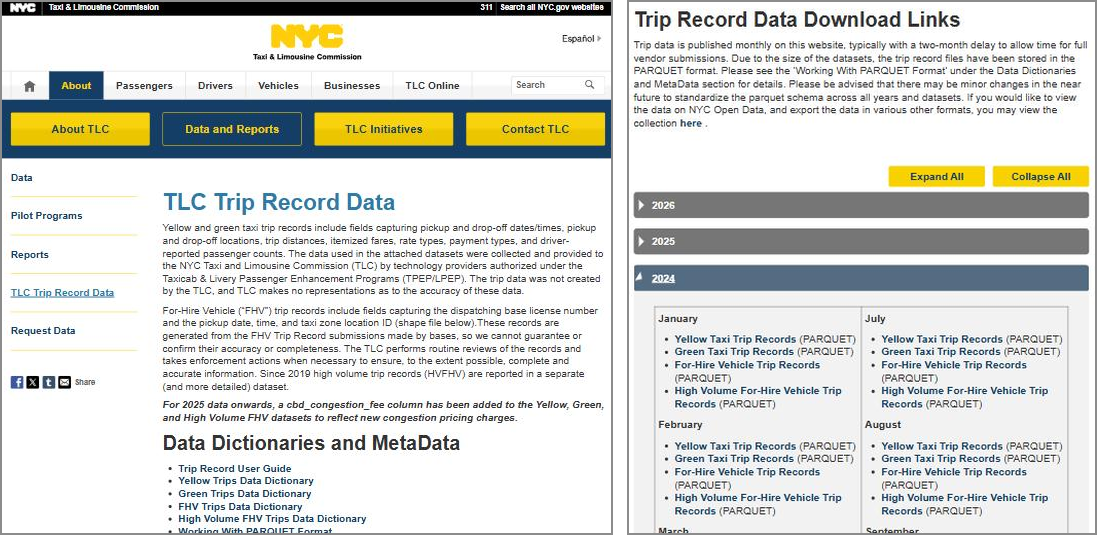
\includegraphics[width=\columnwidth]{figures/tlc_website.png}
\caption{The data source: the TLC Trip Record Data page on \texttt{nyc.gov}. Left:
description of the records and the data dictionaries. Right: monthly download links
(2024 expanded), one Parquet file per month and service type. Screenshots taken in
November 2026.}\label{fig:tlc}
\end{figure}

These questions are \emph{data parallel}: every record can be processed on its own and
the partial results combined by summation. They are therefore a natural fit for
MapReduce~\cite{dean2008mapreduce} and its in-memory successor
Spark~\cite{zaharia2012rdd,zaharia2016spark}, which split the input across machines
and run the same function on every split. What is less obvious is \emph{how much}
adding machines helps for data of this size, and when it stops helping.

\subsection{Problem statement and objectives}
Given the TLC yellow-taxi records, compute (i)~trip demand per zone and hour of day,
(ii)~the top-$N$ pickup$\rightarrow$drop-off routes, and (iii)~average fare and
credit-card tip rate per distance band; then measure how the run time changes when the
same work is spread over one, two, three or four machines. Our objectives are to:
\begin{enumerate}
  \item install and operate a Hadoop (HDFS, YARN, MapReduce) and Spark cluster in
        Docker containers, on one host and on a public cloud;
  \item implement the three analytics jobs as Python MapReduce programs;
  \item compare a single computer (one container) with multiple containers in
        run time, speedup and efficiency, and explain the differences.
\end{enumerate}

\subsection{Contributions}
\begin{itemize}
  \item A reproducible cluster: one Docker image and a Compose file for a master and
        1--4 workers with \emph{equal, capped} CPU and memory, plus scripts that run
        the full benchmark unattended.
  \item One Python implementation of each job, reused unchanged by Hadoop Streaming,
        Spark RDDs and a single-process baseline, with outputs cross-checked for
        equality.
  \item A strong- and weak-scaling study over six data sizes (1--24 months), 1--4
        workers and five execution engines on one host, repeated on Azure VMs:
        786 timed runs in total, plus a 48-run cache experiment.
\end{itemize}
